%\section{Simulation}
\subsection{Simulation}
\begin{frame}{System Dynamics}
	\framesubtitle{Simulation}
	\begin{figure}[H]
		\centering
		$m_1 = 1\,\left[\mathrm{kg}\right]$, $m_2 = 2\,\left[\mathrm{kg}\right]$, $L = 0.4\,\left[\mathrm{m}\right]$, $\omega = 3\pi\,\left[\mathrm{\frac{rad}{s}}\right]$, $x_0 = \left(\begin{array}{c c}
		1 & 0
		\end{array}\right)^T$\\
		\begin{figure}[H]
			\centering
			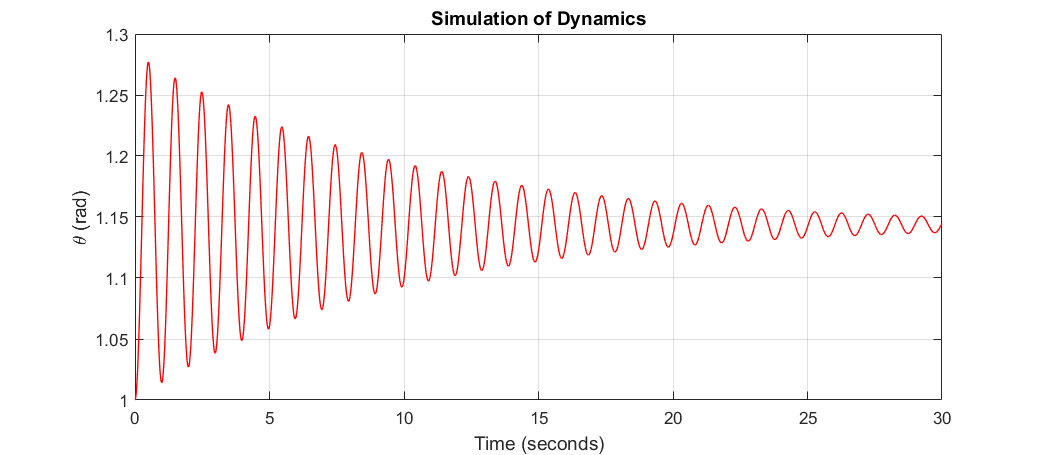
\includegraphics[width=1\textwidth]{pics/simulation.png}
		\end{figure}
	\end{figure}
\end{frame}

%\subsection{SimMechanics}
%\begin{frame}{Simulation}
%	\framesubtitle{SimMechanics}
%	Eventuelle Erfolge mit SimMechanics werden hier dargestellt werden.
%\end{frame}